\documentclass{bioinfo}
\copyrightyear{2015}
\pubyear{2015}
\usepackage{natbib}
\usepackage{xpatch}
\usepackage[toc,page]{appendix}
\usepackage{url}
\usepackage{texpower}

\begin{document}
\firstpage{1}

\title[BCI]{A Study of Brainwave eSensing Activity }
\author[Dhali \textit{et~al}]{Salle Dhali\,$^{1}$}
\address{$^{1}$Department of Computer Science, Malm\"{o} University.\\}
%$^{2}$Department of XXXXXXXX, Address XXXX etc.}

\history{Date 2015-06-04}

\editor{Contact: \href{salledhali@msn.com}{salledhali@msn.com}}

\maketitle

\begin{abstract}

\section{Motivation:}
The  Neurosky Mindwave device allows monitoring the electrical signals generated by the brains neural activities. The easy access of this devices opens a new area of researching fields not only in the gamification and disable people but also to understand the cognitive behavior of human beings. The purpose of this study is to investigate the consistency and effectiveness level of a non-invasive consumer product BCI. We investigate the output of the headset data both in quality and quantity of that gathered data and determine how it could be used for human involved research settings. A sample of two participants in terms of an interview and an interviewer interchanging questionnaires. The cognitive tasks and EEG output signals captured by the participants both attentive and meditation values.

\section{Results:}
The data we collected produces mixed results. The meditation or relaxing level provide a consisting output while the attention level need more to explore due to the nature of every individuals and also the surrounds such as noise, mode distraction levels etc.


\section{Keywords: BCI, Brain activity,EEG,NeuroSky, Attention, Meditation} \end{abstract}

\section{Introduction}

A brain-computer interface (BCI) often calls a brain-machine interface (BMI) is a communication channel between our brain and external devices \citep{wolpaw}. Until the recent years the advancement of Information Technology (IT), cognitive neuroscience and brain signals capturing technologies by external devices both in non/or invasive allow us to interact with human brain directly \citep{wijayasekara}. BCI device capture brainwaves and transform into actions, unlocking new worlds of interactivity. Neurosky  MindWave logs the wearer’s mental state in the form of NeuroSky's embedded properties such as Attention and Meditation with the help of eSense algorithms not an open source platform \citep{larsen}. 

For decades human has fantasized to communicate and interact with machines via thoughts itself and moreover expectation was that the devices will be able to reveal human minds, feelings, meditation and attention as well.
The use of sensors make it possible monitor brains neuron process activities that can relates to certain form of thoughts as for instance how much focused we are in certain objects from an interview to interviewer for get out the thoughts as an analogue values and convert it to digital signals output produced by human brain \citep{Nijholt}.

NeuroSky MindWave also capable to capture the raw brain wave and information about the brainwave frequency (Hz) bands. It can be used with supported video games, research software, improve the quality of disable people's everyday activities also developing applications for enhancing user experience \citep{NeuroSky}. This paper we will investigate how the gathered data from users can be measured for determining the consistency level of both the focusing and easiness levels of the cognitive behavior for researching of human settings.


\section{Aims and Goals}
The objective of this study is to investigate the NeuroSky Mindset, to see how we could operate and integrate it with .NET infrastructure and also how we could get data from it. Moreover, we will try to see if there is any trace of correlation between its claimed states attention and meditation in respect with the test users. The feedback's will be taking care of. Moreover, we will study how BCI could help facilitates simple cognitive recognition events/features in terms of providing cards/questionnaire to users that will be both known and unknown and investigate the level of activities waves at the particular time stamps for determining the focusing and relaxing consistency levels. So the research question will be:\\

\textbf{RQ1:} How the Brainwaves differ in respect with known and unknown objects?

\textbf{RQ2} What are the consistency of those measurements levels regards to focusing and relaxing states?

\section{Literature Review}

Brain–computer interface (BCIs) started with Hans Berger's inventing of electrical activity of the human brain and the development of electroencephalography (EEG). In 1924 Berger recorded an EEG signals from a human brain for the first time. By analyzing EEG signals Berger was able to identify oscillatory activity in the brain, such as the alpha wave (8–12 Hz), also known as Berger's wave \citep{cauvery}.

NeuroSky Mindset is not the most accurate BCI containing only one tiny electrode, it still supports a number of detection such as Attention and Meditation \citep{stonehill}. Moreover, it allows a broader range of raw brain waves data, enabling a more potent signal processing. In addition, as a benefit for gaming experience, it is essentially a wireless headset which can play music, this might enhance the gaming experience by providing surrounded sound of better quality than ordinary loudspeakers \citep{lyu}. It has a very low costs compared to other BCI's makes more affordable. BCI can be used augmented reality than existing experience field of medical treatment by enhancing a game, where a BCI can improve the gaming experience and also to influence the environmental variables \citep{Nacke}. 

Previous research in the same area was conducted by \citep{dietrich} where the question investigates whether a correlation can be made between an EEG system data capturing and a Brain-Computer Interface (BCI).Also researcher \citep{lyu} tries to investigate how game and user experience can be integrated by using this affordable devices such as NeuroSky. Researcher such as \citep{stonehill} also tried to investigate how NeuroSky can be used to improve the cognitive behavior of human by conducting both qualitative and quantitative research in transport system with blinking systems for warning the drivers avoiding accident.


%\pagebreak
\begin{figure}[ht!]
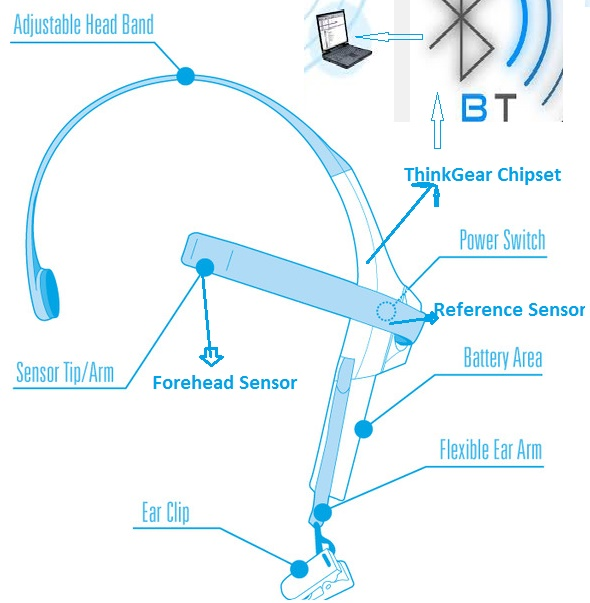
\includegraphics[width=0.5\textwidth]{Neurosky_headset.jpg}
\caption{ System overview includes the key components of MindWave Headset (Adopted \citep{NeuroSky})}
\end{figure}



%\begin{methods}
\section{Methods}

A design science research methodology settings was used to conduct this research paper. To contribute the knowledge we followed the design science research process such as awareness of problem, future suggestions, technical development, discussion/ evaluation and conclusion \citep{vaishnavi}.

We collect the brainwave data of user when asking the questionnaire. The questionnaire was prepared writing in the paper ark and provide it to the interviewer by the interview. The interviewer answered the questions and the brainwaves recorded by tagging the time stamps of every second passes. The interview when used different term that was not included in the questionnaire formulation and how the focusing level at that moment occurs was recorded. We then analysis the brainwave data to see if there is any correlation between mental states regarding attention and relaxing levels. Besides the research tools such as interview we also used other technical methods to capture, analyze and visualize the gathered data.

\textbf{NeuroSky mindset}: The EEG device that is wearable as a regular headphones. It consist of one dry sensor that can be placed on the forehead, left side above the eye (Fp1 position) \citep{stonehill} which is shown in figure 1. It has three dry sensors on the left ear. It has a microchip which pre-process the EEG signal, and transmits that data via Bluetooth. The processing algorithms are not an open protocol, but it does a Fast Fourier Transformation (FFT) on the signal which gives the band powers. However, these powers are scaled and filtered and thus only relative to each other \citep{NeuroSky}.

The mindset have speakers, like a headset, and a microphone, so it can be used for multiple tasks such as game play. The key components that build the MindWave headset for connecting with the Bluetooth for PC and the device itself and how the ThinkGear generic chip set that process the signal data acquired by the headset and also through its own Bluetooth module can be seen in the system overview figure 1.

Mindset provides a raw unfiltered brainwave measurement. The raw data can be used by researchers and developers to make own algorithm to measure mental states such as attention and meditation which are available as input data for games and educational applications. Raw data includes alpha waves, beta waves, gamma waves, delta waves and theta waves \citep{larsen}. The data flows from headset sensors to the processing algorithm (FFT) is shown in figure 2.


\textbf{Bluetooth:} A Bluetooth module is included in the mindset headset. It communicates with the PC/ Mac devices with the Bluetooth connection to a COM port, makes application and headset device communication for data streaming. BrainWave is the windows form application and it has a graphical user interface, shows in figure 5 in Appendices section, which allows headset connection and displays the raw data and also the emotion senses data which will be recorded for analyzing purpose.


\textbf{Mindset SDK interface:} There are libraries available for Mac/Windows
/Linux based platform and supporting different programming languages such as C++, C\# and Java \citep{NeuroSky}. The interfaces instantiates by the Bluetooth modules between the mindset and computer that makes the communication channel. In this project, we use the .NET wrapper class ThinkGear which take care all the connection, disconnection and receives bytes of all the output data which we write in a separate file as a typed data for string as well as Integer values. 

The SDK provides well documentation, drivers and sample codes for development that allows developers collect Mindset data. We collect the Time stamp and attention and meditation values in every second and the raw data that generates every half seconds such as beta, alpha values we discard those as those are out of scope in this project. The data we collected by using the .NET infrastructure with the object oriented programming language C\#. In Visual Studio 2013 we build the Graphical User Interface for connecting/ disconnecting the TG interfaces and connecting to the COM port for communication channel for collecting the raw data can be seen in figure 5.

\begin{figure}[ht!]
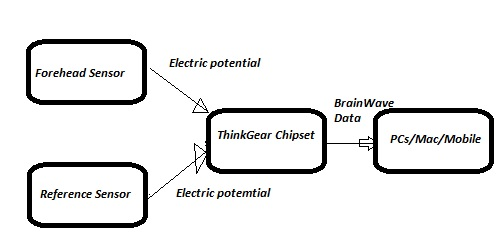
\includegraphics[width=0.5\textwidth]{Data_Flow_Mindset_Computer.jpg}
\caption{Data flow diagram from Mindset headset to computer}
\end{figure}


\textbf{ThinkGear (TG):} TG technology includes the sensor that touches the forehead, the contact and reference points located on the ear pad and the on-board chip that processing all the data. Both eSense Meters and raw data are
calculated on the ThinkGear chip. These data are then sent to the computer
through Bluetooth.

The MindWave headset, MindWave SDK integrating with MS .NET, COM communication with the applications sequence are shown in figure 6.


%\end{methods}


\section{Result}
The data generated by the MindWave kit we captured it in a Comma Separated Value (CSV) file format and store it locally in our computer. As we mentioned eSense algorithm capture data in every single seconds shows in Figure 4 in Appendices. We then export that file to an another API to analyze the result as a visualization shows in Figure 3. From the figure we can see that when asked unknown answer the Attention level goes high but that not happen all the time as we get feedback from the users after the interview session. The Attention level is moderate (under 80) most of the time even the question was not known the level was not goes high. It may be the distraction, bored question or the noise that causes decreasing the attention level. However, the meditation level was quite satisfactory in respect with the attention level as we can see that the level is high when the attention level is in between values  40 to 60 (timestamp between the 4 seconds interval 16:41-16:45) shows in figure 3.

\begin{figure}[ht!]
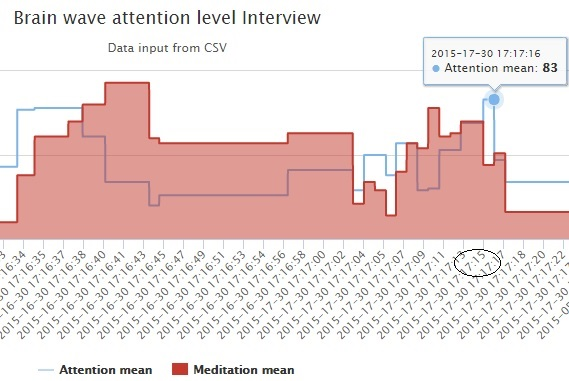
\includegraphics[width=0.5\textwidth]{AttentionLevelWith_Meditation.jpg}
\caption{Analyzing of the Attention (Blue)and Meditation (Red) values ranges between 0-100 in the Y-axis}
\end{figure}

\section{Discussion}
This paper aims to answer the research questions about how the brainwaves differ in respect with known and unknown answers for a question. We can presume that in certain time span the focusing level goes very high over 80 however after a while it goes down as perhaps the user might feel bored or not have a good reason to argue for that question. However we see that the consistency for meditation level is promising. The time of testing the average value was moderate around 40-60.
However, like other BCI's technologies MindWave set also has its drawback.
It is difficult to establish a perfect connection between the headset
sensor and the users forehead. Also the latency is high as it requires sometime to make establish between the devices. This limitations we would like to address during demonstration and mentioned to the test users. As headset capture the mental states data every seconds so large datasets established however it allows developers and researchers access of more data to analyze the results. 

\section{Conclusion}

In this paper, we aimed to understand the brainwave activity captured by the affordable devices NeuroSky Mindset and investigate how the attention and meditation values correlates in regards to different objects which are known and both unknown. We also aimed to understand the activities by reading those values when they are focused or relaxed. BCI is a new emerging area to explore which is now extend from patients rehabilitation to other area  of research such as game, user experience and understanding cognitive behavior for human settings. We developed an application to store the brainwave data and visualize and analyze it for investigating the attention and meditation levels od participants. 

During our study we noticed that when the users are feeling bored, there is a decrease level of attention values. The attention value is lower than normal value below 60 for bored, distracted participants. It may raise the difference  between unknown answers that decrease the level of attention as user can't focus what to think for answer that question. Other possibility could be the participants lose the focus because they do not understand the questionnaire formulation.

However, we can draws the conclusion that relaxation levels are consistent in our study. The level was high when focus level was as high as 93 when the level of attention was almost 20. More research will give clear option in this area as the devices generates Big data so we have the opportunity to analyze and synchronize data from multiple users at the same time to see the correlation about the different brainwaves.

\section{Future works}
The data we gathered from the users we analyzed it visually in two different imputed files by using the JSFiddle. The data from the same time stamp with different users can be a future work to implement a system where the data can be synchronized in a single file and analyze it. The video streaming we captured in the camera we didn't implement it in our application. This option includes with some static images where known and unknown objects also mention to the users not to look at ceratin objects and how it generate their brain activities can be a future object to investigate.

\section*{Acknowledgement}
We would like to thank all of our stakeholders for this project their contributions and valuable feedback. We would also like to thank our teachers Daniel Spikol, Sven Packmohr and Nils Ehrenberg for their supervision and support.


%\bibliographystyle{natbib}
%\bibliographystyle{achemnat}
%\bibliographystyle{abbrv}
%\bibliographystyle{bioinformatics}
%
\bibliographystyle{unsrt}
%
\bibliography{document.bib}
\newpage
\begin{appendices}
\chapter{Data Collection CSV file, Application GUI, Sequence Diagram, }

\begin{figure}[ht!]
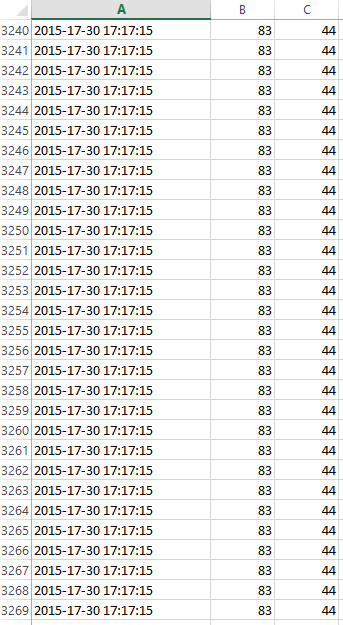
\includegraphics[width=0.5\textwidth]{BrainWaveDataToCSV}
\caption{Data record in every seconds from MindWave kit, whre cell A,B and C represents the Timestamp, Attention and Meditation values}
\end{figure}

\begin{figure}[ht!]
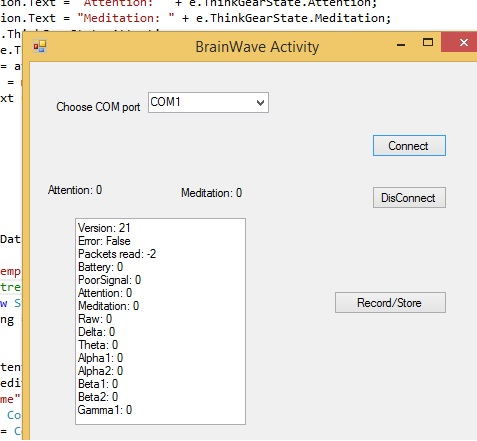
\includegraphics[width=0.5\textwidth]{GUI_BrainWave.jpg}
\caption{BrainWave Application in VS with MindWave power Off mode}
\end{figure}

\begin{figure}[ht!]
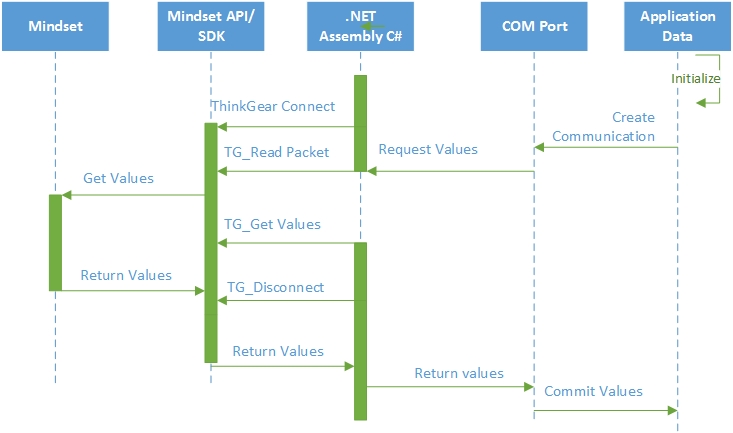
\includegraphics[width=0.5\textwidth]{Drawing2.jpg}
\caption{Sequence Diagram of MindWave headset, Mindwave SDK and program Application}
\end{figure}


\end{appendices}

\end{document}